\section{VALIDATION AND VERIFICATION}\label{sec:valid}
It is important to remark that some of the procedures that are going to be present in this section are doing twice. Model $1$ uses the data of all the month provide by Neuromédica that we are going to refer to it as the model $1$ and the other one, i.e model $2$ only uses the data of the last of the month.

Although a model cannot be formally validated, we use different forms of validation: black and white validation. White validation is a more empirical procedure, checking that numerous parts of the model operate properly.  On the other hand, black-box validation is intended to check the general behavior of the model, comparing it with the real system using confidence intervals \cite[Ch. 12]{robinson2004simulation}. 

Furthermore, the waiting time for each of the type of customers was tested with the waiting time obtained in the simulation by the Kruskal-Wallis test.

\subsection{White-Box Validation}
We used several white-box validation methodologies since the model in consideration does not have a lot of components. The first test consists of submitting the model to extreme conditions, such as:
\begin{itemize}
\item One attendant.
\item All modules open.
\end{itemize}


The results using one attendant in the Model $2$ are shown in Figure \ref{fig:one_att_one_week} which presented the total number of people that are waiting in the system for one week. This validates the model since it shows that the waiting times augment during the day when it is used only one attendant.  It can see a repetitive pattern in the graphic, this represents when the system is closed, which provides a general idea that the model is working well.

\begin{figure}[H]
    \centering
    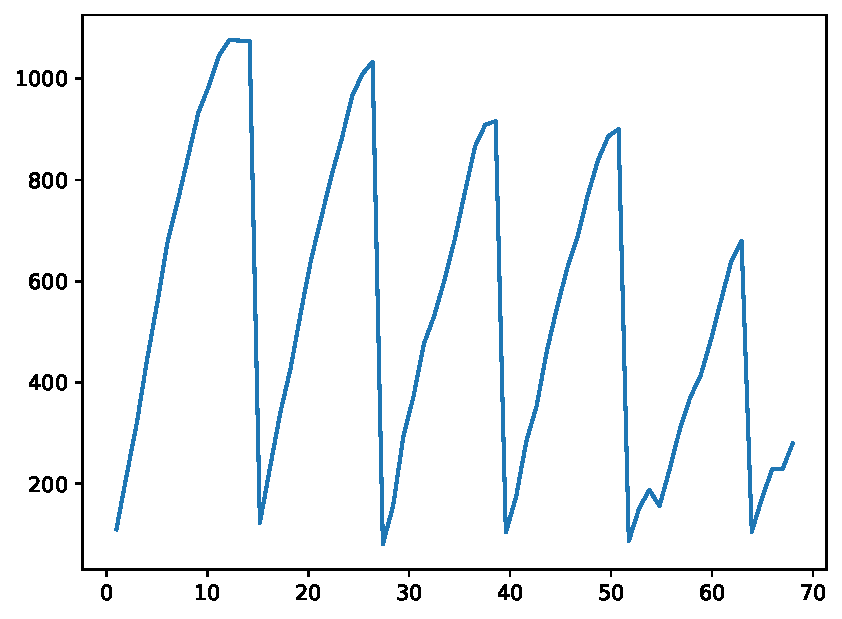
\includegraphics[scale=0.6]{files/validation.pdf}
    \caption{Number of patients for each hour with one attendant}
    \label{fig:one_att_one_week}
\end{figure}

In Figs. \ref{fig:model_1_vali}, \ref{fig:model_2_vali} it can be seen two different box plots for each of the model compared with the one obtained in the data set. In both, the first box plot determines one in which the test assured that both where homogeneous and the second box plot is non-homogeneous.

It is important to see that in the second model, more outliers are generated. This was done with the intention of simulating more human behavior, as the attendants generally have some erratic behavior which which worsen the system. On the other hand, the second model has a lot more cases in which the data is homogeneous making it preferable to use.

Lastly, it is important to remark that the second model is not homogeneous in the type of client "Farmacia General" which is the one with the biggest waiting times in the real system. Hence, it is known that although the model works better than the previous one, it is not a fully working simulation model.

\begin{figure}[H]
        \centering
        \begin{subfigure}[b]{0.475\textwidth}
            \centering
            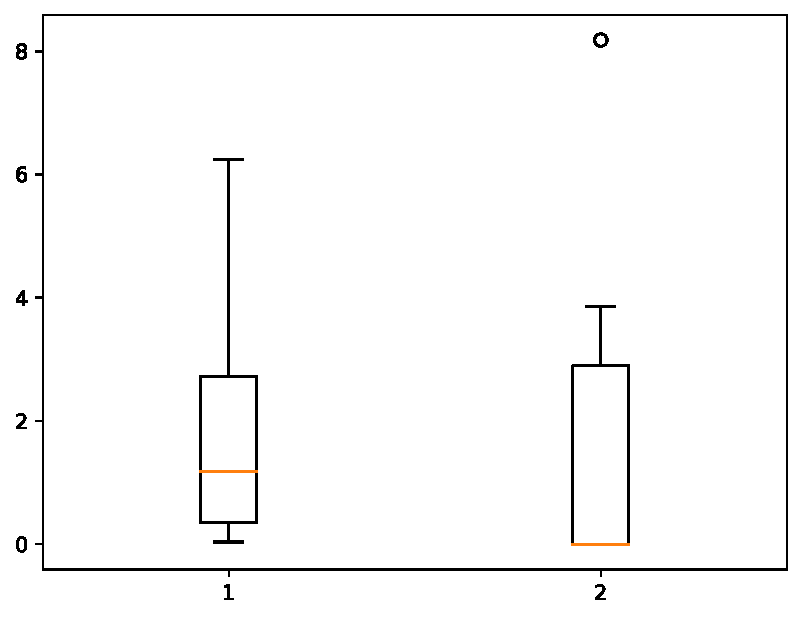
\includegraphics[scale=0.5]{files/test-for-wednesday-for-type-pref-confirmacion-de-citas.pdf}
            \caption{Homogeneous (Pref Confirmación de citas).}
            \label{fig:model_1_homo}
        \end{subfigure}
        \begin{subfigure}[b]{0.475\textwidth}   
            \centering 
            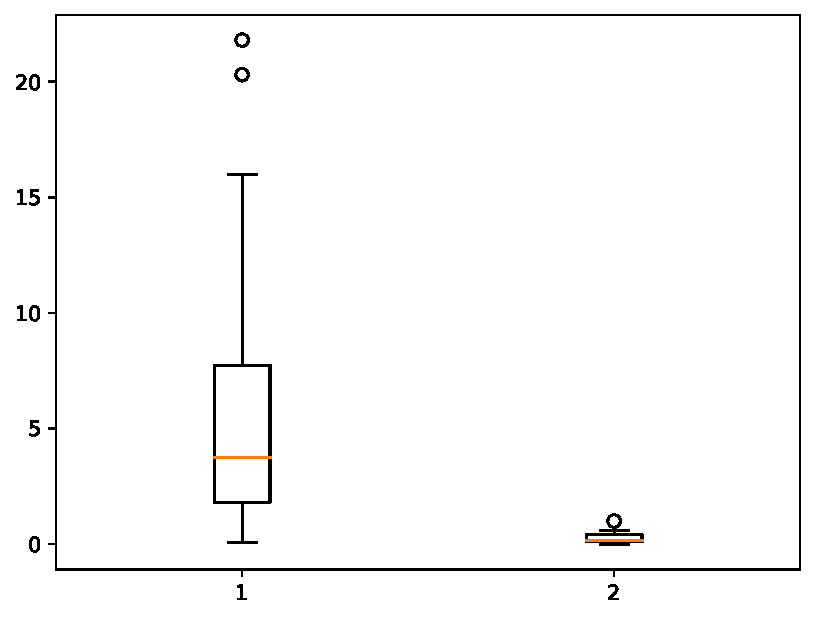
\includegraphics[scale=0.5]{files/test-for-wednesday-for-type-tramites-despues-de-citas.pdf}
            \caption{Non-Homogeneous (Trámites después de Citas).}
            \label{fig:model_1_no_homo}
        \end{subfigure}
        \caption{Boxplots validation for Model $1$.}
        \label{fig:model_1_vali}
\end{figure}


\begin{figure}[H]
        \centering
        \begin{subfigure}[b]{0.475\textwidth}
            \centering
            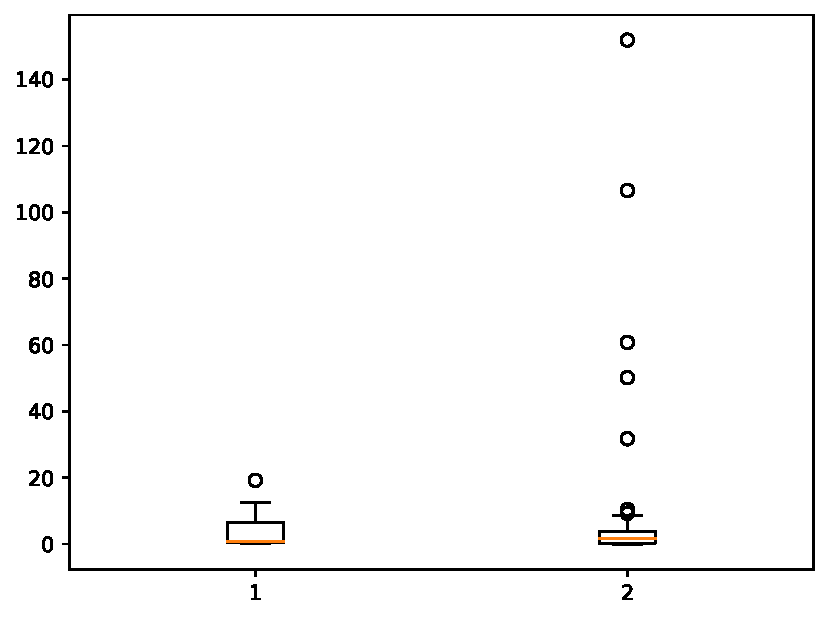
\includegraphics[scale=0.5]{test-for-thursday-for-type-tramites-despues-de-citas.pdf}
            \caption{Homogeneous (Trámites después de Citas).}
            \label{fig:model_2_homo}
        \end{subfigure}
        \begin{subfigure}[b]{0.475\textwidth}   
            \centering 
            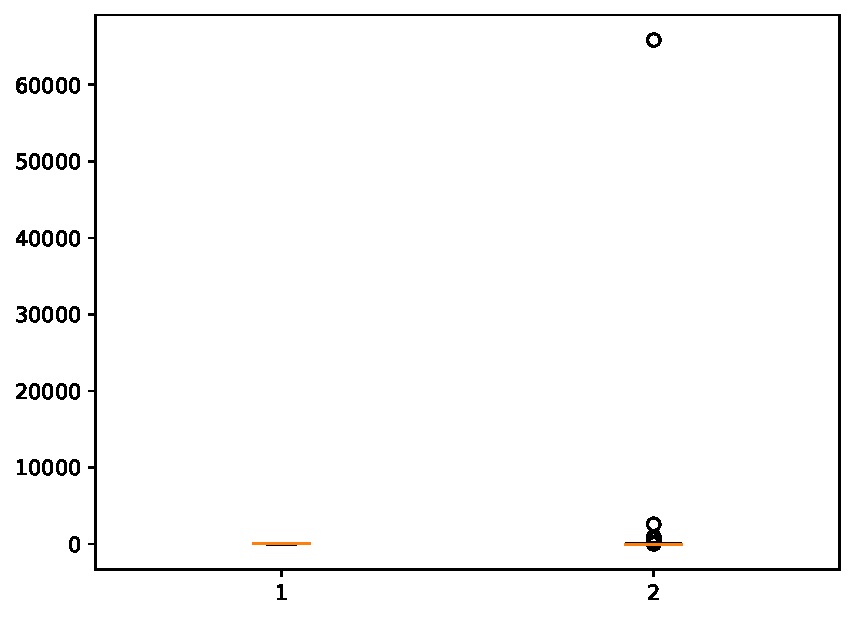
\includegraphics[scale=0.5]{test-for-friday-for-type-farmacia-general.pdf}
            \caption{Non-Homogeneous (Farmacia General).}
            \label{fig:model_2_no_homo}
        \end{subfigure}
        \caption{Boxplots validation for Model $2$.}
        \label{fig:model_2_vali}
\end{figure}


Furthermore, whilst the model was being implemented, multiple runs were performed to check initial conditions, arrivals/attention distributions and general proper behavior of the system.

\subsection{Black-Box Validation}
As previously stated, the general behavior of the model can be analyzed using the corresponding confidence interval to check the difference of the means. The formula its calculation is \cite[pp. 218]{robinson2004simulation}:

\begin{equation}
        \bar{X}_{\mathrm{S}}-\bar{X}_{R} \pm t_{2 n-2, \alpha / 2} \sqrt{\frac{S_{S}^{2}+S_{R}^{2}}{n}}
        \end{equation}
\begin{equation*}
\begin{aligned} \bar{X}_{\mathrm{S}} &=\text { mean of simulated output data } \\ \bar{X}_{\mathrm{R}} &=\text { mean of real system output data } \\ S_{\mathrm{S}} &=\text { standard deviation of simulated output data } \\ S_{\mathrm{R}} &=\text { standard deviation of real system output data } \\ n &=\text { number of observations (this must be the same for the } \\ & \text { simulated and real system data) } \\ t_{2 n-2, \alpha / 2} &=\text { value from Student's } t \text { distribution with } 2 n-2 \text { degrees of freedom and } \\ & \text { a significance level of } \alpha / 2 \end{aligned}
\end{equation*}

So the obtained result has more sense, it is going to be used the type of pacient "Confirmacion de citas". This was chosen because this type of pacient is the one that the simulation is capable of characterizing. Hence, all experiments are going to be analyzed through the waiting time of this customer.

With this test, it was found that the interval for the difference of the means is:

\begin{equation}
    [-3.74976, 1.57127]
\end{equation}